\chapter{Results}
\label{chap:results}

[brief introduction of the chapter]

\section{Smart Contract Interactions}
\label{sec:smart_contract_interactions}

Like mentioned, the blockchain is a public ledger that stores all the transactions that are made, so we can see all the interactions with the smart contracts. We deployed the smart contracts on a testnet, so that we don't have to use real funds. This way we can simulate what would happen on the mainnet without any risks or cost. This was done with Foundry, like mentioned before, and we created some scripts to populate the system to be able to see it on the blockchain. These scripts deploy the smart contracts, adds an organizer, creates a few events, and adds some packages to each.

For each network there is an explorer that allows us to see all the transactions that are made, and the Figure \ref{fig:system_transactions} shows what it looks like. What we're seeing is the page of the interactions with the main smart contract and we can see when the contract was deployed, the adding of an organizer to the system, and the creation of the 3 events.

\begin{figure}[H]
    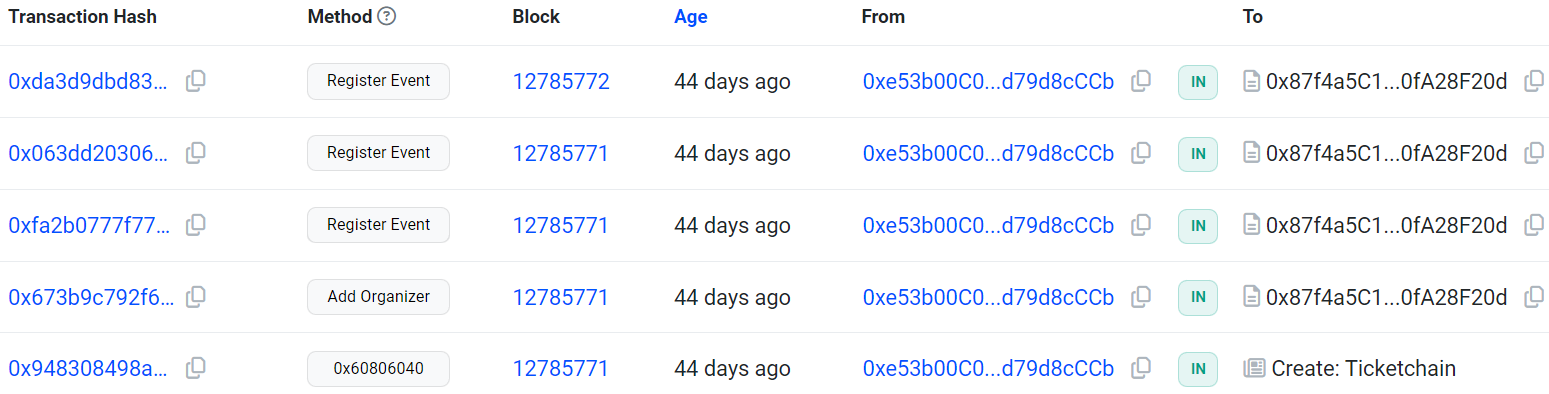
\includegraphics[width=\textwidth]{System transactions.png}
    \centering
    \caption{System Transactions}
    \label{fig:system_transactions}
\end{figure}

If we go into one of the events creation, we can see the details of the transaction and its logs. On the details we see the information of the transaction itself, like the hash, the status, and the gas information. This gas information is the cost of the transaction, and it's paid in the network's currency. The logs are the events that are emitted by the smart contract, and in this case we see the event of the creation of the event, like the Figure \ref{fig:event_transaction_logs} shows. Not to confuse the events that are emitted by the contract and the event that is created by the organizer.

\begin{figure}[H]
    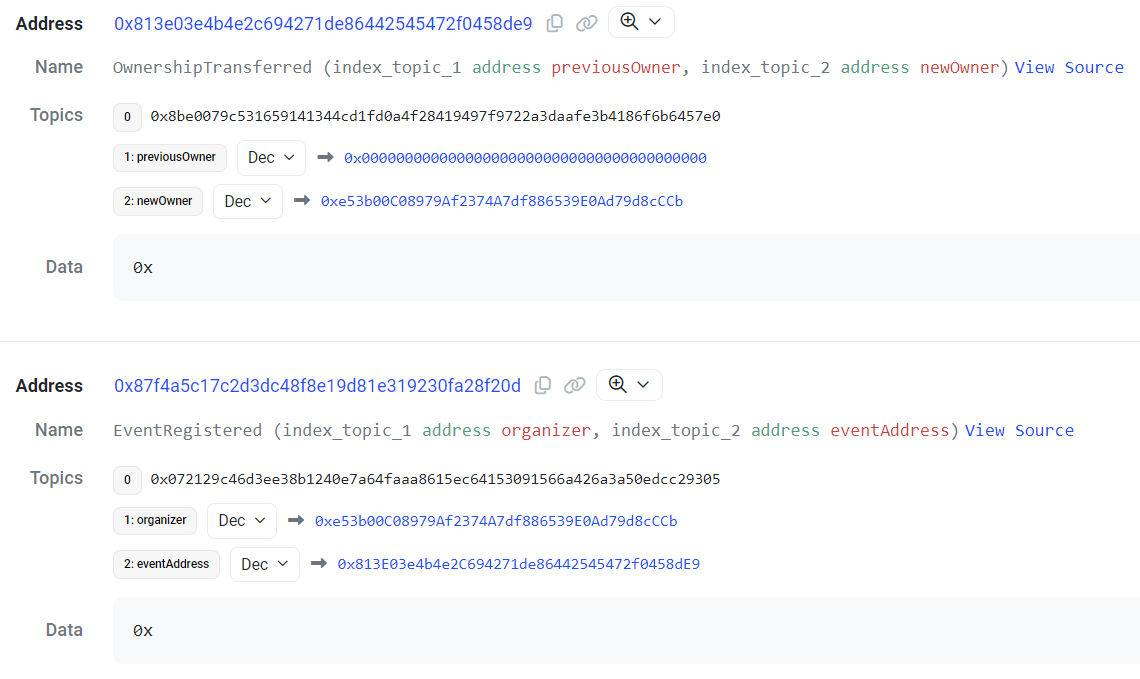
\includegraphics[width=\textwidth]{Event transaction logs.png}
    \centering
    \caption{Event Transaction Logs}
    \label{fig:event_transaction_logs}
\end{figure}

This shows two events being emitted and the first is the transfer of ownership. This is because we set the owner of the event contract to be the organizer, so that he has full control over it. The second is the creation of the event, and we can see the organizer that created it and the address of the event. When we search for that address we see its interactions, like the Figure \ref{fig:event_transactions} shows. Analyzing its entries we see the addition of 3 packages, 2 additions of validators, one entry of buying tickets and one ticket validation. The added packages were done by the initial script to populate the event, the rest of the interactions were done manually.

\begin{figure}[H]
    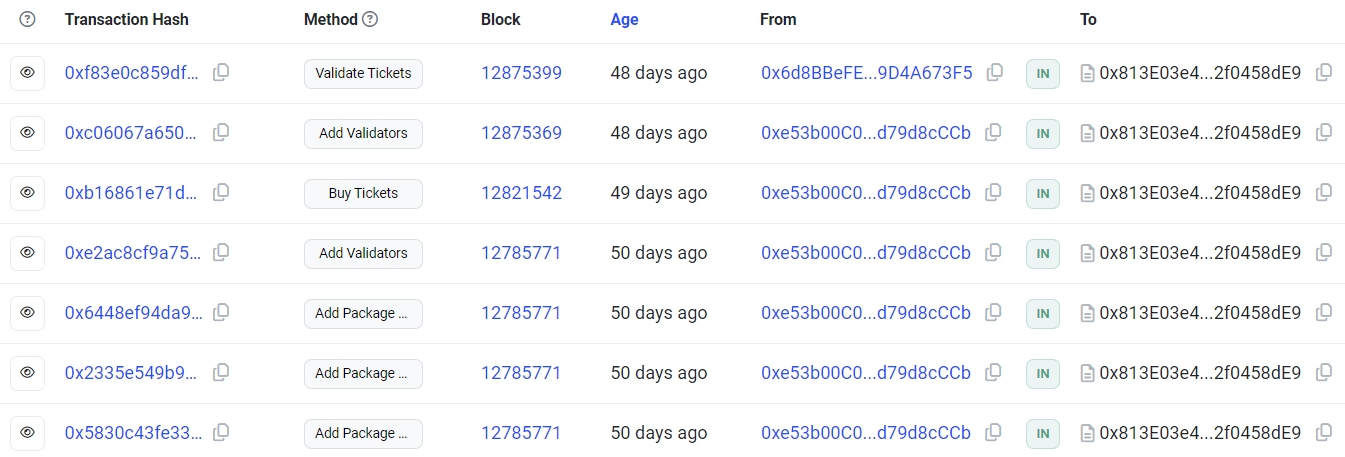
\includegraphics[width=\textwidth]{Event transactions.png}
    \centering
    \caption{Event Transactions}
    \label{fig:event_transactions}
\end{figure}


The script also does one extra thing to helps us interact with the contracts. When deploying, there's an extra step called verifying the contract. This is optional and is only useful to be able to see the code in the explorer. What happens behind the scenes is the entire code is compiled and sent to the network to be stored, and the explorer has an option of associating it with the readable code. For this to happen, we need to prove that the code matches the compiled one and that we have permission to do so, by also proving that we own the private key of the address that deployed the contract. What this process essentially does is we can read the entire code and interact with it directly on the explorer. Not to forget that, not doing this process, the explorer still has the bytecode of the contract, so someone that knows how to decode it can still see the code, since everything in the blockchain is public.

What's more useful for us is to be easier to interact with it from the explorer directly and the Figure \ref{fig:event_read_functions} shows a few of the functions that we can call on the smart contract, separated by the ones that are read-only and the ones that change its state, meaning the ones that have to be signed and payed for.

\begin{figure}[H]
    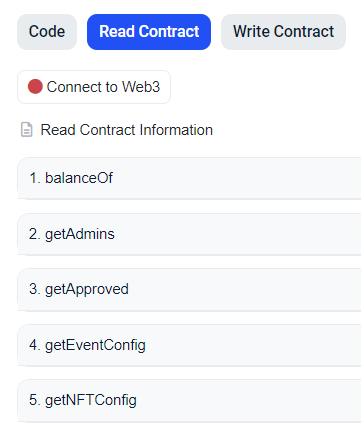
\includegraphics[width=\textwidth/2]{Event read functions.png}
    \centering
    \caption{Event Read Functions}
    \label{fig:event_read_functions}
\end{figure}

This is where we can see the details of the event, cause we made the getters for each of the structs that are important. As an example, we can check the packages configuration by calling the getter. The Figure \ref{fig:package_config} shows the result of calling the getter of the package configuration, but in this case it shows as a tuple, because the explorer doesn't understand the custom structs made by us. Still we can see its contents organized like shown in the Section \ref{subsubsec:packageconfig_struct}, showing the name, the description, the price (in wei, the smallest unit of ether), the supply, and the bool saying if the NFTs share the data.

\begin{figure}[H]
    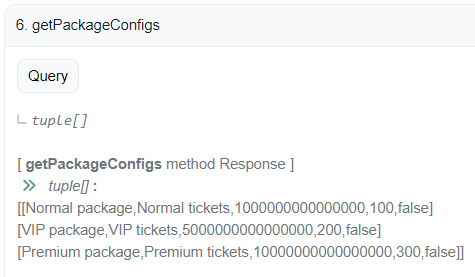
\includegraphics[width=\textwidth/2]{Package config.png}
    \centering
    \caption{Package Config}
    \label{fig:package_config}
\end{figure}

\section{Mobile Application}
\label{sec:mobile_application}

[show application]
[show smart contract interactions on the blockchain]